\documentclass[10pt,a4paper]{article}

\usepackage[margin=18mm]{geometry}
\usepackage[T1]{fontenc}
\usepackage[utf8]{inputenc}
\usepackage{microtype}
\usepackage{graphicx}
\usepackage{booktabs}
\usepackage{amsmath}
\usepackage{natbib}
\usepackage[hidelinks]{hyperref}
\graphicspath{{Images/}}

\title{\textbf{Contention-Aware Expert Parallel Load Balancing\\
in Mixture-of-Experts Serving in vLLM}\\[2mm]
\large Executive Summary}
\author{Wu Cao, 11036000\\
Advisor: Prof. Qiaolun Zhang\\
Co-advisor: Prof. Massimo Tornatore}
\date{Academic Year 2026--2027}

\begin{document}
\maketitle

\begin{abstract}
Mixture-of-Experts models distribute sparse expert computation across devices.
Expert Parallel Load Balancing periodically changes expert placement to remove
runtime hotspots, but applying a placement requires transferring expert weights.
In asynchronous mode, these transfers share network resources with live
inference. This work formulates the resulting contention problem, develops a
lightweight migration-batching algorithm, integrates it into vLLM, and evaluates
it on a four-node deployment. In the final A/B experiment, batching improved
output throughput by 2.28\%, reduced every reported TTFT, TPOT, and end-to-end
latency percentile, and reduced head-node NIC P99 by 10.24\%. The implementation
was reviewed and merged into the upstream vLLM project.
\end{abstract}

\section{Motivation and problem}

Sparse MoE layers activate only a subset of their experts for each token, which
increases parameter capacity without activating every parameter
\cite{shazeer2017moe,fedus2021switch}. Under expert parallelism, expert weights
are placed on different ranks and tokens are dispatched to the selected experts.
The resulting load is input dependent. EPLB observes expert usage and periodically
computes a new placement, potentially replicating popular experts.

A synchronous migration pauses inference, so completing all transfers as quickly
as possible is the natural objective. Asynchronous EPLB is different: inference
continues while weights move in the background. Posting every point-to-point
transfer together can create a short NIC burst that interferes with token
dispatch, result collection, and other distributed inference communication.
The objective is therefore not only to finish migration quickly, but also to
protect foreground serving while migration is active.

The offline formulation represents each coalesced source--destination flow $p$
with size $w_p$. Binary variable $x_{p,b}$ assigns it to batch $b$, while $y_b$
indicates whether that batch is active. For routed link $e$, the migration load is

\begin{equation}
  L_{e,b}=\sum_p w_p f_{p,e}x_{p,b}.
\end{equation}

The model first minimizes the worst modeled inference time,

\begin{equation}
  T_{\mathrm{infer}}^*=\min T_{\mathrm{infer}}, \qquad
  T_{\mathrm{infer}}\ge
  T_0\left(1+\frac{L_{e,b}}{C_e(1-\rho)}\right),
\end{equation}

then minimizes $\sum_b y_b$ while preserving the primary optimum. This strict
two-stage order avoids choosing an arbitrary weight between inference protection
and batch overhead. In the illustrative eight-rank hotspot, the ILP reduces peak
normalized link utilization from 1.50 to 0.50 and modeled inference time from
4.75 to 2.25, using three batches. Figure~\ref{fig:summary-ilp} shows the
topology, the unbatched hotspot, and the resulting schedule.

\begin{figure}[t]
  \centering
  \begin{minipage}{0.32\textwidth}
    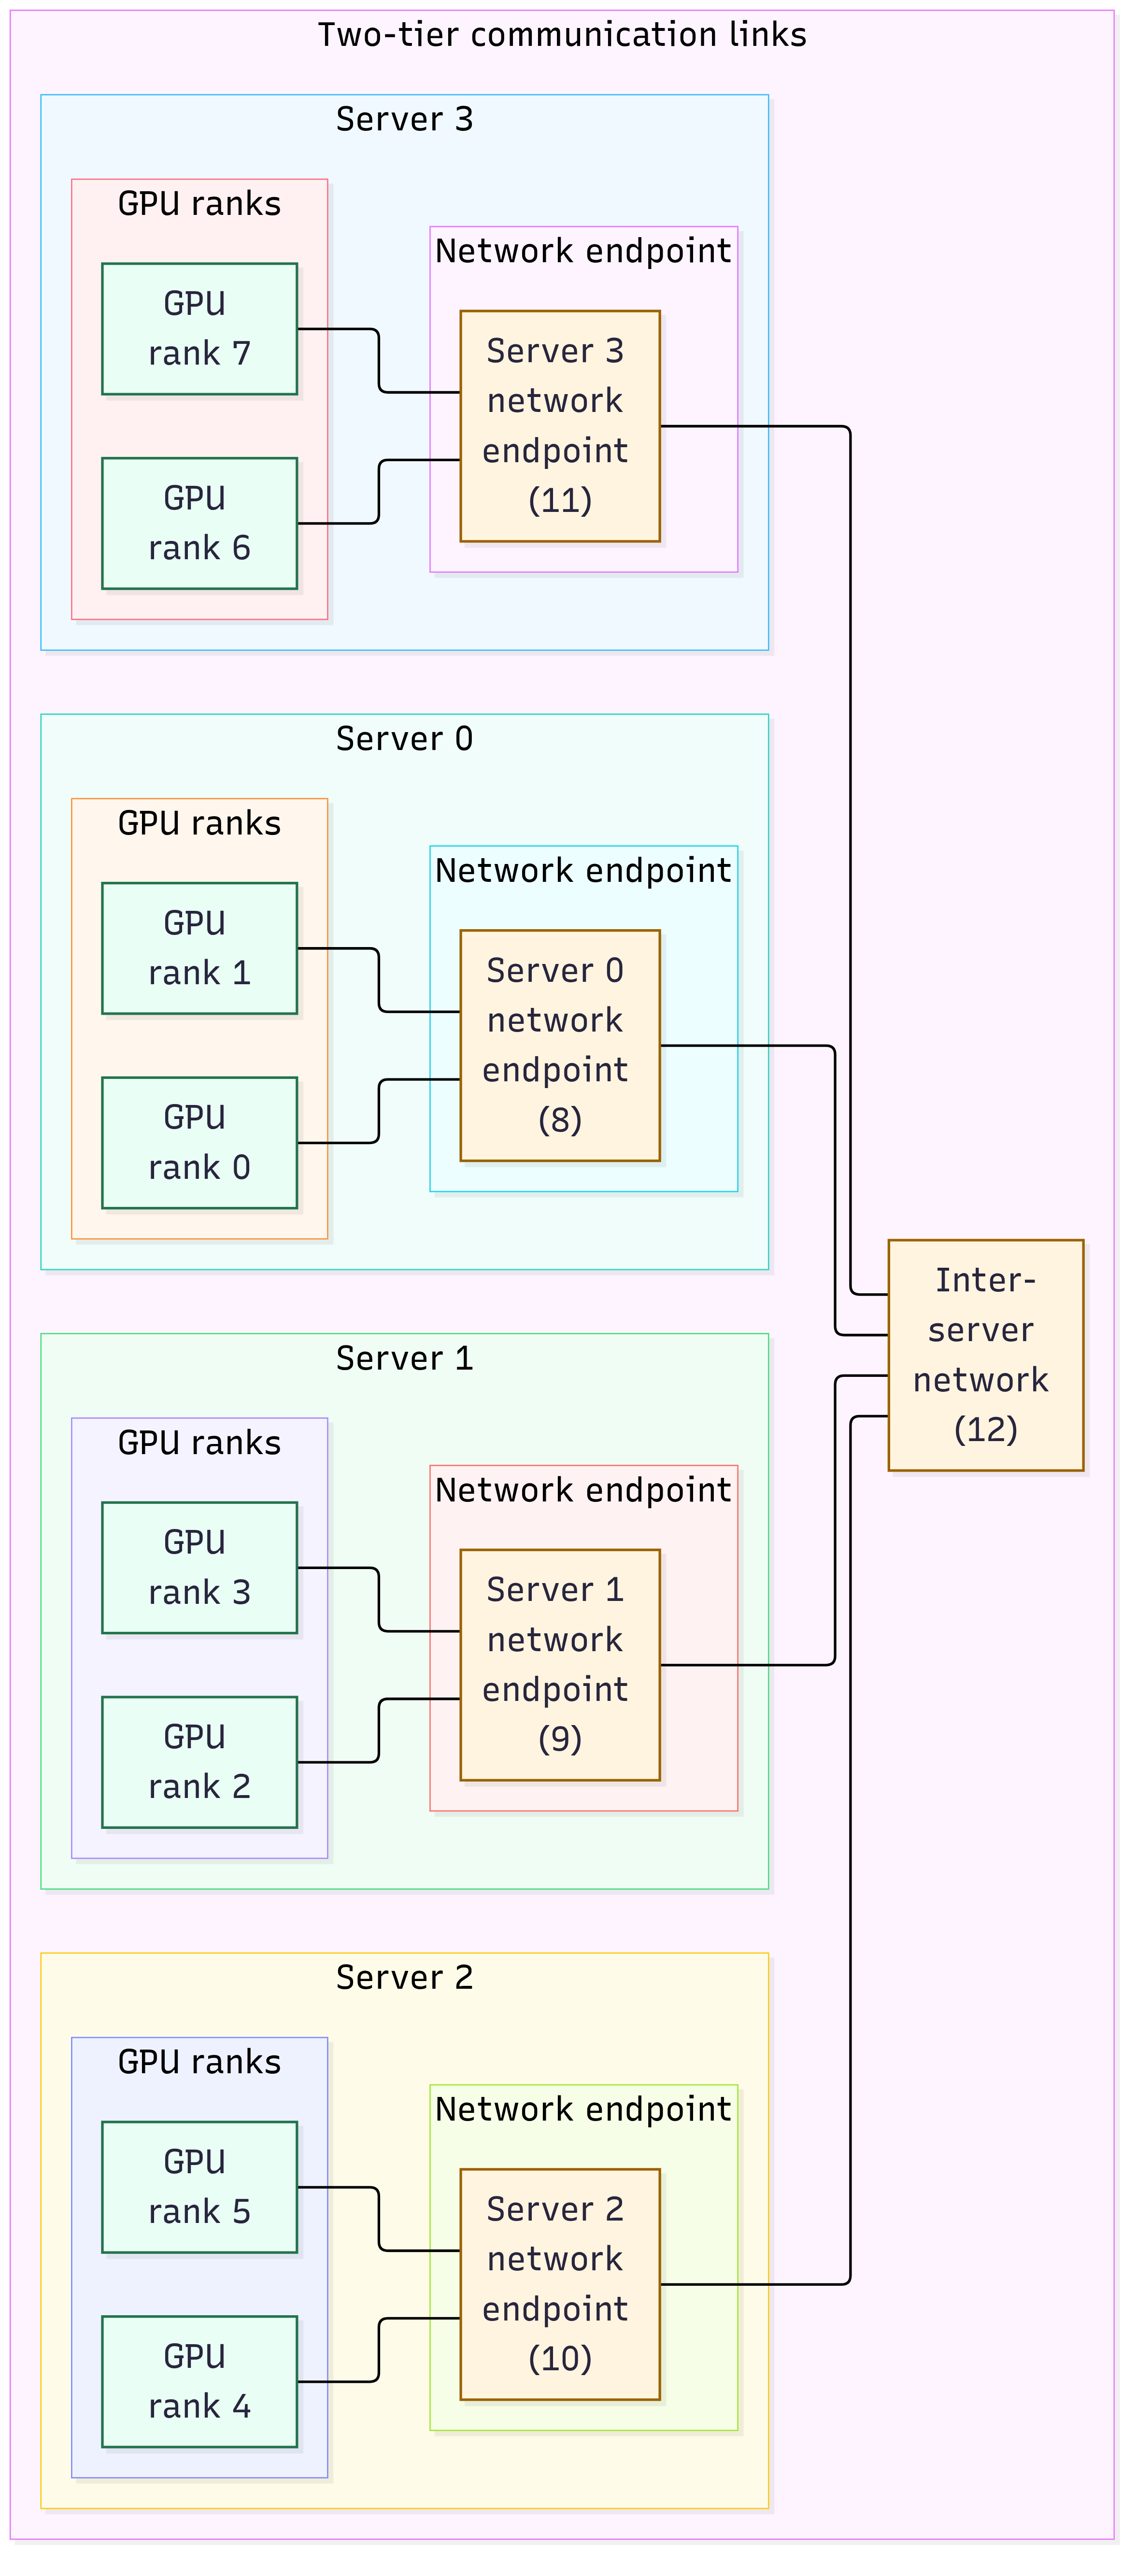
\includegraphics[width=\linewidth]{example_hotspot_links.png}
  \end{minipage}\hfill
  \begin{minipage}{0.32\textwidth}
    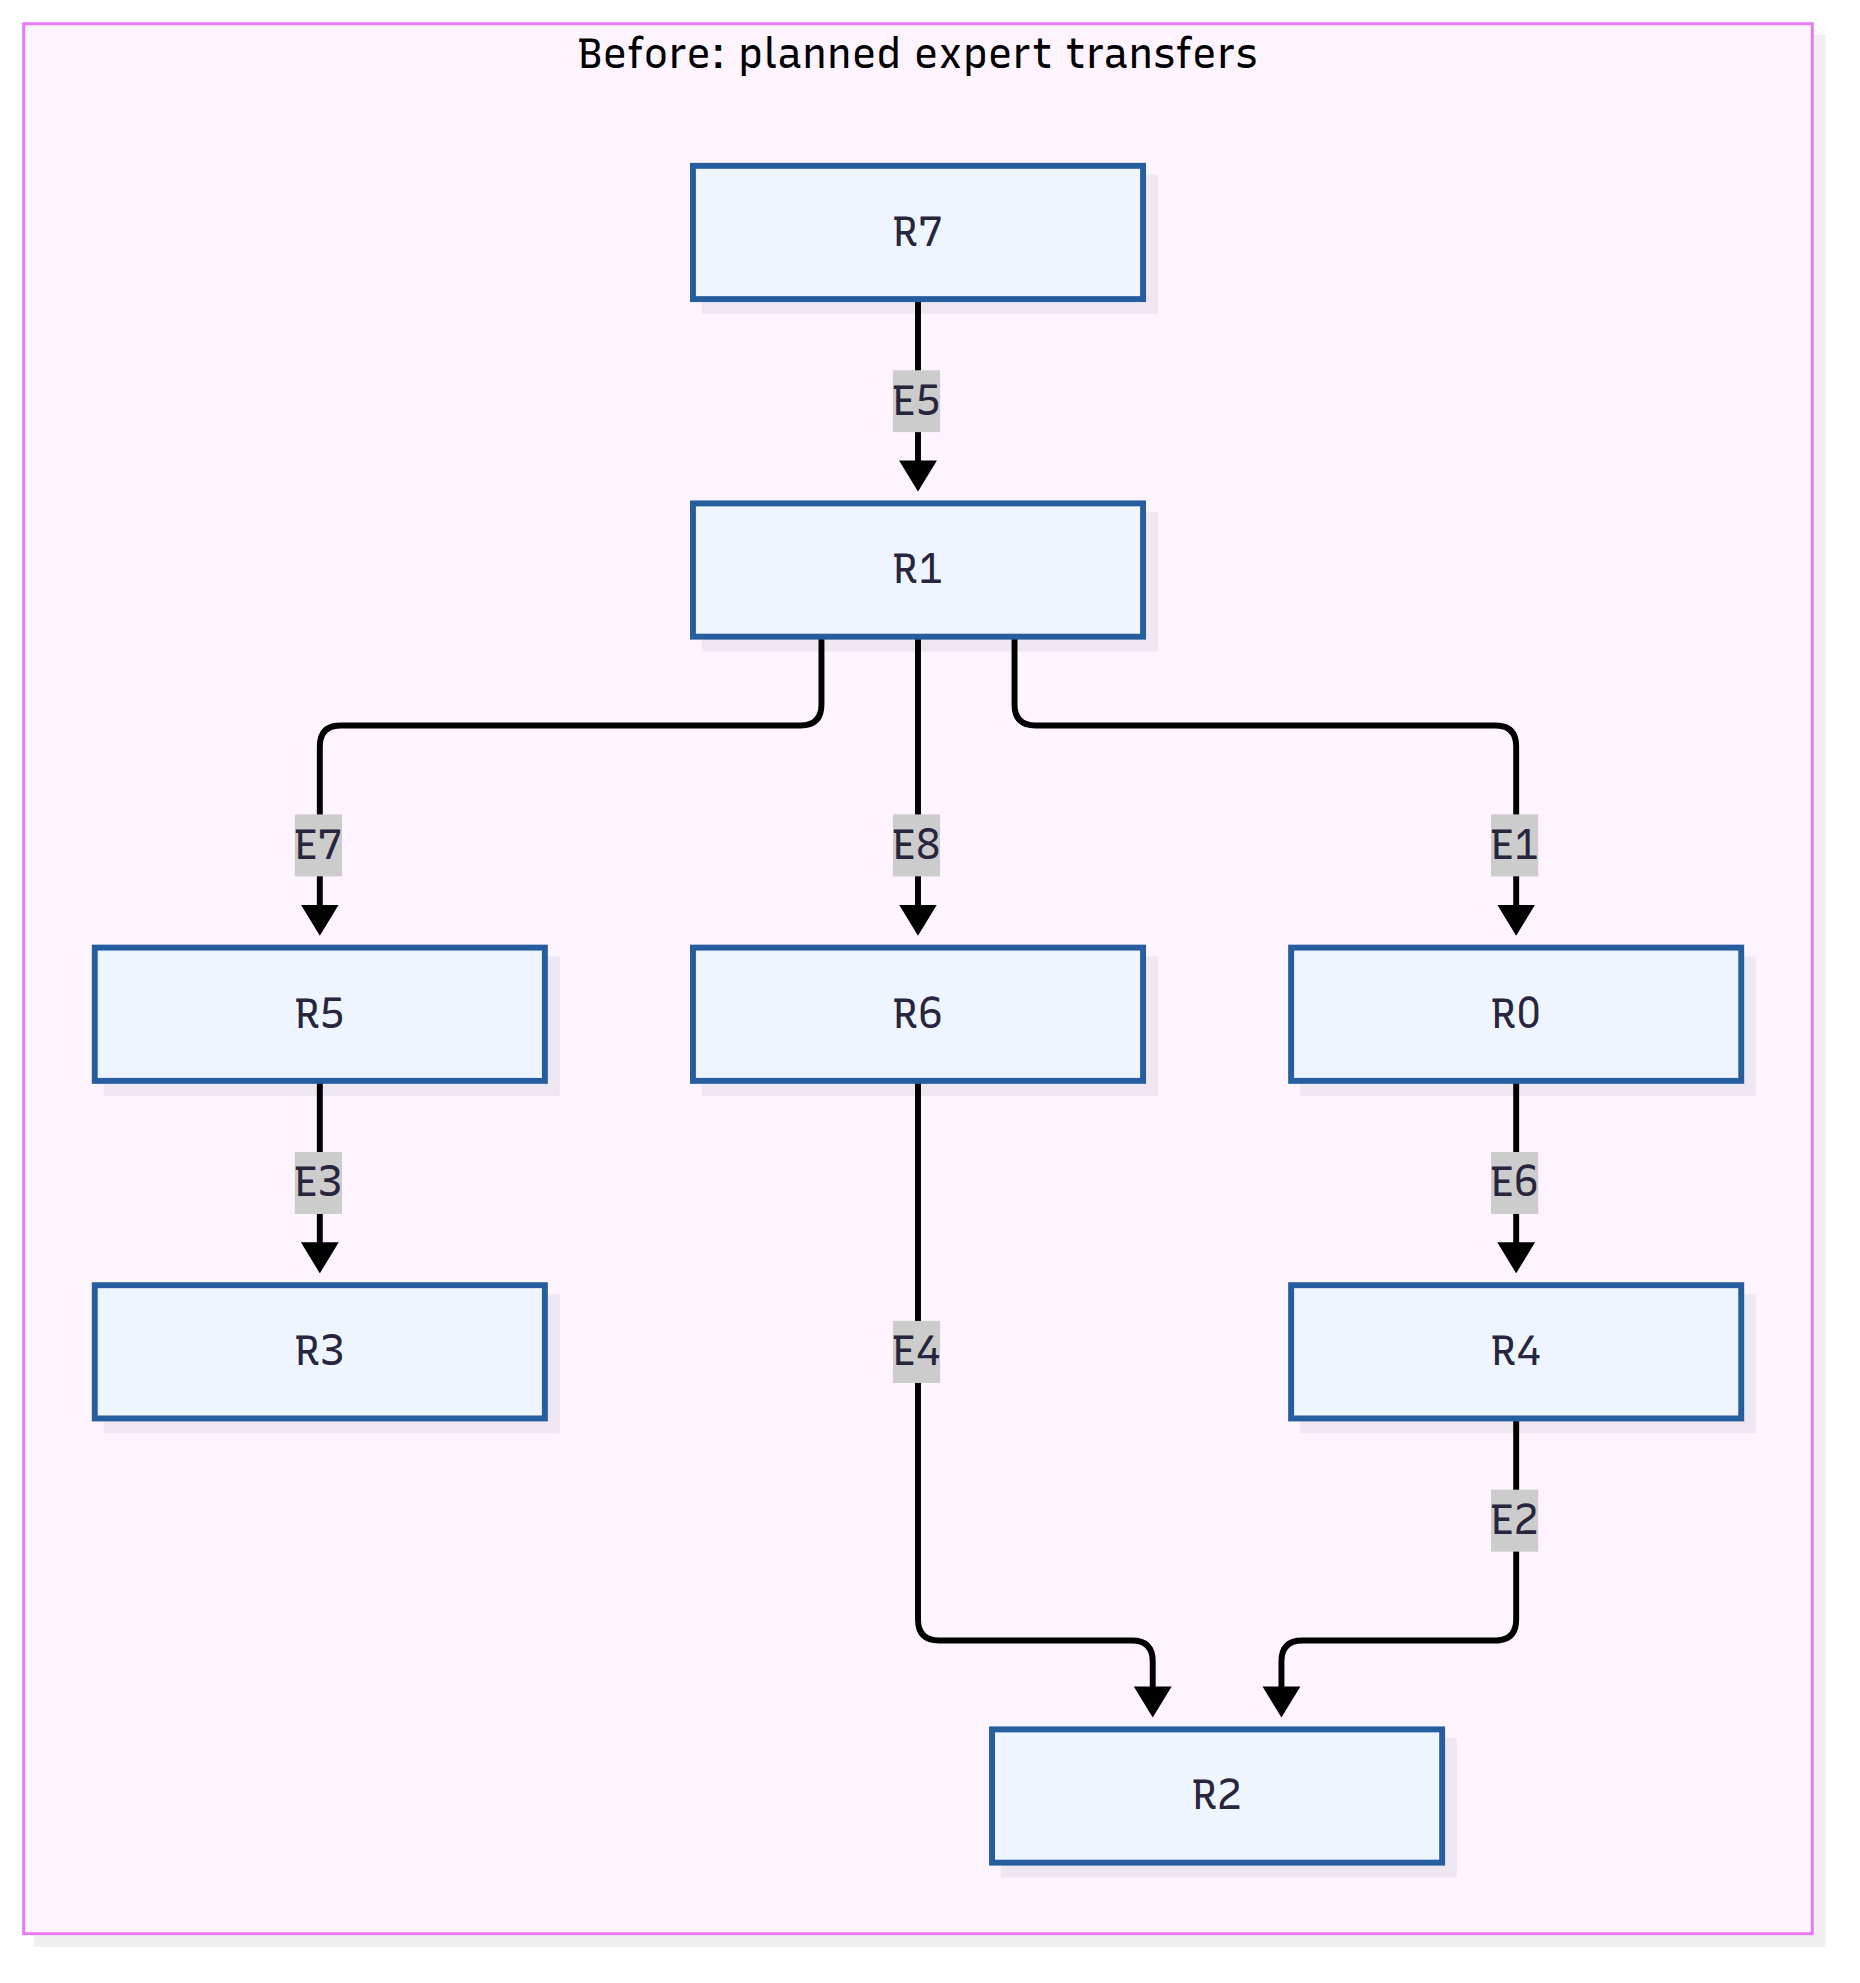
\includegraphics[width=\linewidth]{example_hotspot_before.png}
  \end{minipage}\hfill
  \begin{minipage}{0.32\textwidth}
    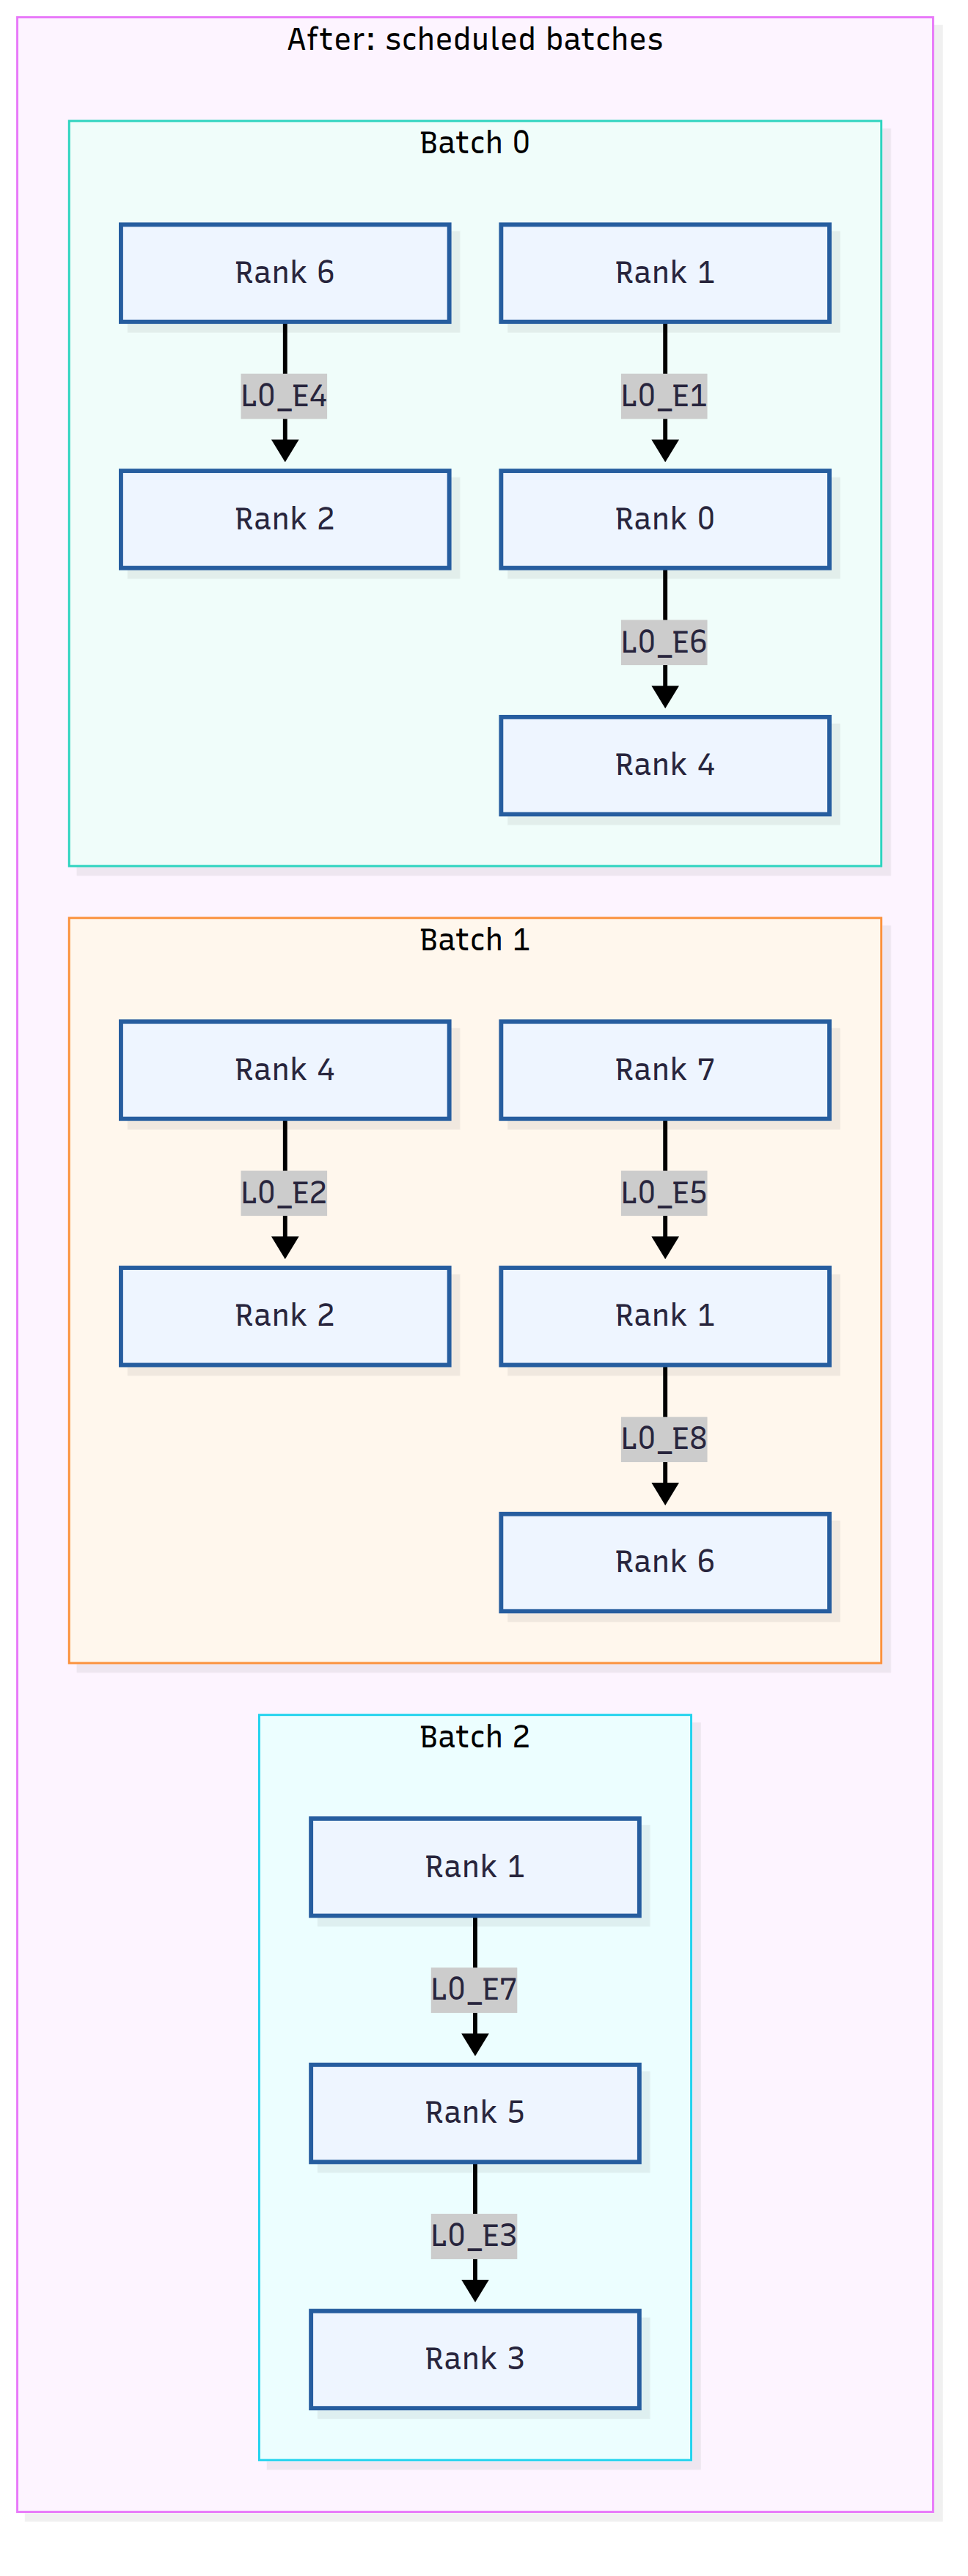
\includegraphics[width=\linewidth]{example_hotspot_after.png}
  \end{minipage}
  \caption{Illustrative topology, unbatched migration hotspot, and the
  three-batch ILP schedule.}
  \label{fig:summary-ilp}
\end{figure}

\section{Production methodology}

The online scheduler avoids a solver and uses deterministic greedy grouping.
Remote migrations are first coalesced by ordered rank pair. A flow with endpoints
$(s,d)$ has bit mask $(1\ll s)\lor(1\ll d)$. It is placed in the first batch whose
used-rank mask is disjoint; otherwise a new batch is created. Thus, each batch is
a matching in the rank communication graph. Independent rank pairs retain
parallelism, while one rank never communicates with several migration peers in
the same batch.

The implementation preserves the legacy placement, source assignment, local-copy
semantics, and layer activation order. It prepares all layer schedules in one CPU
call per rebalance cycle, but expert weights are still transferred layer by layer.
For NIXL, every batch restores the layer transfer context, posts only that batch's
sends and receives, and calls the communicator. The feature is opt-in and can
operate only with asynchronous EPLB; the synchronous path remains unchanged.

The baseline is the legacy path, which posts all remote transfers for a layer
before one communicator execution. The proposed condition changes only the
migration-batching configuration flag. This isolates scheduling from placement,
model, workload, and backend changes.

\section{Evaluation}

The final experiment uses four Ubuntu 22.04.5 nodes, one Quadro RTX 6000 GPU per
node, and 10~Gb/s Ethernet without RDMA. Qwen3-30B-A3B-Instruct-2507 runs
with tensor parallel size four, expert parallelism, Ray, and NIXL over UCX/TCP.
The benchmark contains 500 successful requests at concurrency 32, with a
300-token random prefix, 200 additional input tokens, and 300 output tokens.
Prefix caching remains enabled. Each condition is one independent run, so the
percent changes are descriptive rather than confidence-bound estimates.
Table~\ref{tab:summary-e2e} reports the complete comparison, and
Figure~\ref{fig:summary-e2e} visualizes the signed improvements.

\begin{table}[ht]
  \centering
  \small
  \caption{Final asynchronous A/B result. Latencies are in milliseconds.}
  \label{tab:summary-e2e}
  \begin{tabular}{lrrr}
    \toprule
    Metric & Off & On & Improvement \\
    \midrule
    Output throughput (tok/s) & 31.54 & 32.26 & 2.28\% \\
    TTFT P50 / P99 & 49180.71 / 75740.25 & 48599.04 / 74756.17 & 1.18\% / 1.30\% \\
    TPOT P50 / P99 & 828.53 / 1007.82 & 812.44 / 999.01 & 1.94\% / 0.87\% \\
    E2E P50 / P99 & 303462.69 / 322184.88 & 293821.76 / 317351.61 & 3.18\% / 1.50\% \\
    Head NIC P99 (MB/s) & 599.81 & 538.40 & 10.24\% \\
    \bottomrule
  \end{tabular}
\end{table}

\begin{figure}[ht]
  \centering
  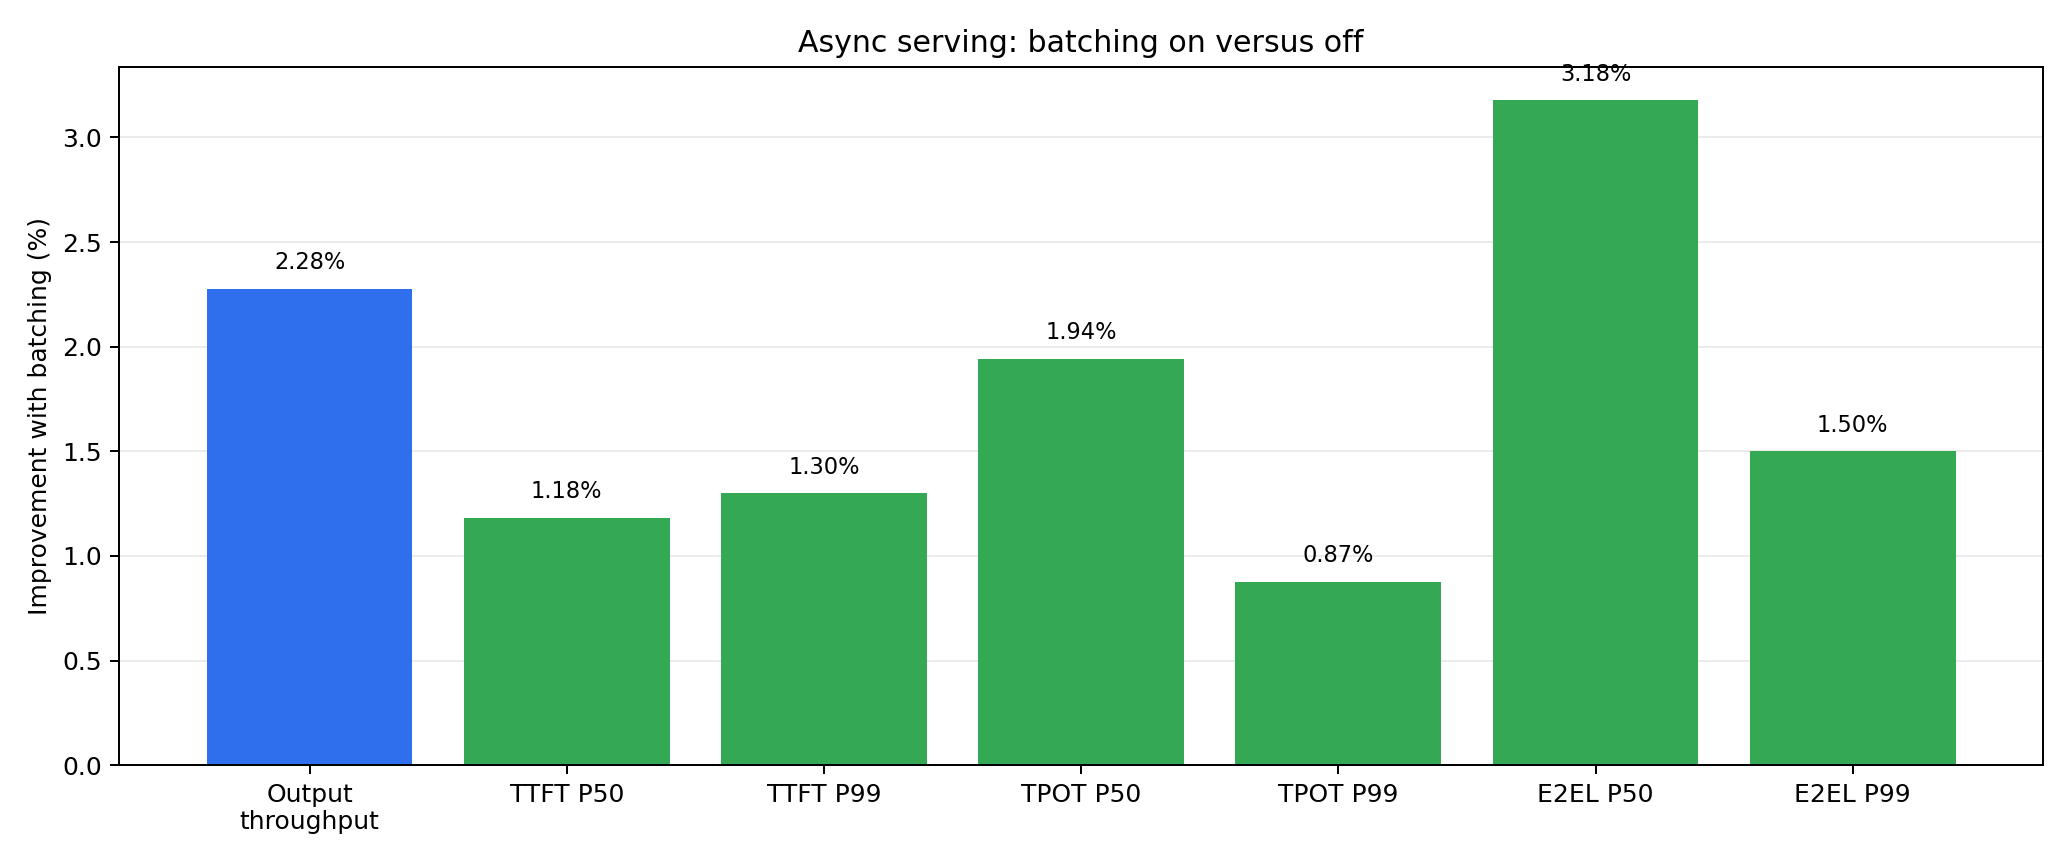
\includegraphics[width=0.88\textwidth]{e2e_improvement.png}
  \caption{Signed relative improvement with migration batching enabled. Positive
  values denote higher throughput or lower latency.}
  \label{fig:summary-e2e}
\end{figure}

The NIC metric is obtained independently from one-second RX and TX byte counters
on the head node. Its lower P99 supports the intended mechanism, but the study
does not attribute individual packets to migration or inference. The workload is
synthetic, the off run preceded the on run, and only one cluster and backend are
evaluated. These limitations prevent a universal performance claim.

Scheduler overhead is measured separately with NVTX-only Nsight Systems traces.
Each range covers schedule construction for all 48 MoE layers. All ranks record
34 cycle-wide calls; the largest cumulative cost is 302.081~ms. The clean
A/B run saves 105.932~s, so the conservative cost-to-saved ratio is 0.285\%.
The profile and serving experiment are separate, so this ratio is a scale
comparison rather than a causal decomposition.

\section{Conclusions}

Asynchronous expert migration should be evaluated as part of serving rather than
as an isolated transfer benchmark. The offline model shows why more migration
batches can reduce foreground interference even when migration takes slightly
longer. The production design turns this observation into a deterministic,
dependency-free scheduler with explicit communicator boundaries and a safe
opt-in configuration. In the evaluated deployment, throughput, TTFT, TPOT,
E2E latency, and NIC tail traffic all improve. Future work should repeat and
randomize experiments on server-class GPUs and RDMA fabrics, measure every node,
and adapt the per-rank concurrency limit to observed network headroom.

\bibliographystyle{abbrvnat}
\bibliography{Thesis_bibliography}

\end{document}
